\chapter{Applications and experimental results}
\label{c:results}

\WIP

\section{Examples}

Here we show examples for the program:

\subsection{Genomic sequences}

\todo[inline]{make an example}

\subsection{Event sequences}

To see whether it would be plausible to analyze event sequences we generated a dataset of 5000 sequences of length 20 to 50. The events [\R{A},\R{B},\R{C},\R{D},\R{F},\R{G},\R{H},\R{I},\R{X},\R{Y},\R{Z}] in the dataset are non-uniformly distributed and additionally there is an error event \R{E}, which will happen if there is a "trigger pattern" \R{X.*Y.*Z}. Examples of the sequences:

\begin{file}
# without errors
AIBBFCACCADAHABXCHCG
GBACDBHBDAIBHYDIHAAADAFAHFGGDBFFYFZBFBAGDIDDX
CAGZHGBAXHFIGBAFBIABDYBABBFDBAFGGAAAAHHC
CGDCHHAAAABFBDBCHBBFGICDBGGDGCDFIFADCA
# with errors
ADDDBBCYDFCCHXFDDXBAYDYBHACAZE
DXFDIHBXYDBFGGCBHAYBDHZE
IXBBXHBBACYCFHADHGFDACDHCGYABYBHADZE
AHAFFFGABIXBCAYCBBHBDCDDXZE
\end{file}

It is easy to notice the distinguishing \R{ZE} part, but the \R{X.*Y.*} part is very hard to notice, even when you know that it is there.

To prepare the dataset we extracted sequences into a separate file. Since there can be a lot of patterns by chance we use the whole dataset as a background. This allows us to compare the count of matches in the errors and the whole dataset. If the pattern occurs in both datasets at the same frequency, it is most doesn't distinguish the error dataset.

\begin{file}
pattern      errors      all            ratio      p-value
A.*Z         330/343     1706/5000      2.818      4.952-126
B.*Z         329/343     1676/5000      2.860      1.041-126
X.*G.*Z      254/343     654/5000       5.659      5.511-132
Y.*B.*Z      256/343     596/5000       6.258      1.954-142
X.*Y         343/343     1771/5000      2.822      9.879-147
X.*F.*Z      274/343     717/5000       5.568      2.409-147
X.*C.*Z      285/343     758/5000       5.478      7.304-156
X.*D.*Z      281/343     718/5000       5.701      4.570-156
A.*A.*Y.*Z   250/343     452/5000       8.055      1.304-158
G.*Y.*Z      265/343     515/5000       7.494      1.656-166
F.*Y.*Z      272/343     522/5000       7.588      1.639-174
X.*A.*Z      305/343     811/5000       5.478      1.798-176
X.*B.*Z      304/343     785/5000       5.641      1.540-178
D.*Y.*Z      281/343     557/5000       7.347      1.066-180
C.*Y.*Z      285/343     584/5000       7.107      1.056-181
B.*Y.*Z      292/343     610/5000       6.971      2.370-187
A.*Y.*Z      300/343     616/5000       7.092      3.163-198
X.*Z         343/343     1054/5000      4.740      1.276-215
Y.*Z         343/343     805/5000       6.204      1.009-249
X.*Y,*Z      343/343     343/5000       14.537     0
\end{file}

As we can see this \R{X*Y*Z} pattern can be found very easily. We picked 20 best patterns based on p-value, which was calculated according to hypergeometric distribution.

This example is an ideal situation for the problem and the conclusions should be verified against real world data.

\subsection{Text patterns}

As an example how text patterns could provide useful feedback is to run it on a chapter of thesis. It could find overused words and phrases. To test this claim we ran the algorithm on Chapter \ref{c:implementation}.

To prepare the text we separated each sentence to a separate sequence. Then we removed all the non-textual characters and replaced them with spaces. The text was then converted to lowercase. We could additionally stem the text, but it didn't provide any useful improvements for this text.

We use a group $"bind" = [and, or, if, then, else, the, a, an, my]$ do define words that do not carry much meaning.

As a starting point we searched patterns that may have group symbols and are at least 4 patterns long. We limited the output to 10 results:

\begin{file}
matches  pattern
2        this means that the
2        a practical implementation spexs2 for
2        a practical implementation spexs2
2        discuss a practical implementation spexs2
2        discuss a practical implementation
2        discuss a practical implementation spexs2 for
2        discuss (bind) practical implementation spexs2 for
2        discuss (bind) practical implementation
2        discuss (bind) practical implementation spexs2
2        for pattern discovery in
\end{file}

Repetition of such long word sequences looks very interesting. Further investigation revealed that there was a sentence that was rewritten and the previous version wasn't removed. After removing the repeating sentence we reran and also lowered the pattern length limit to 3.

\begin{file}
matches  pattern
5        the configuration file
4        a lot of
3        this means that
3        in the configuration
3        means that the
3        there are only
3        in (bind) configuration
3        pattern discovery in
3        we can use
3        of (bind) pattern
2        into (bind) configuration file
2        in (bind) configuration file
2        pattern discovery in sequences
2        into the configuration file
2        for pattern discovery in
2        this means that the
2        in the configuration file
2        be the best
2        go is a
2        the algorithm is
\end{file}

We see repetitions such as "this means that", "in the configuration", "we can use" and "pattern discover in", which suggests we can improve the text in such places. So it can find rather simple patterns. Usefulness of the algorithm for such natural language processing tasks should be further examined.

\section{Performance measurements}

To verify that the parallelization improves the performance we need to see a speedup when using multiple cores. As a comparison we also compare with the original spexs. The exact versions used were \emph{spexs2@6b14edd} compiled with \emph{go1.1rc3} and \emph{spexs.0.2.a01}.

For performance analysis we used 400,000 random protein sequences with length 12. Limited number of wildcards to 3 and searched all patterns with at least 5 matches in the dataset. We calculated the average of 5 runs for \emph{spexs} and average of 3 runs for \emph{spexs2}.

\begin{figure}[H]
\makebox[\textwidth][c]{%
\subfloat[]{%
	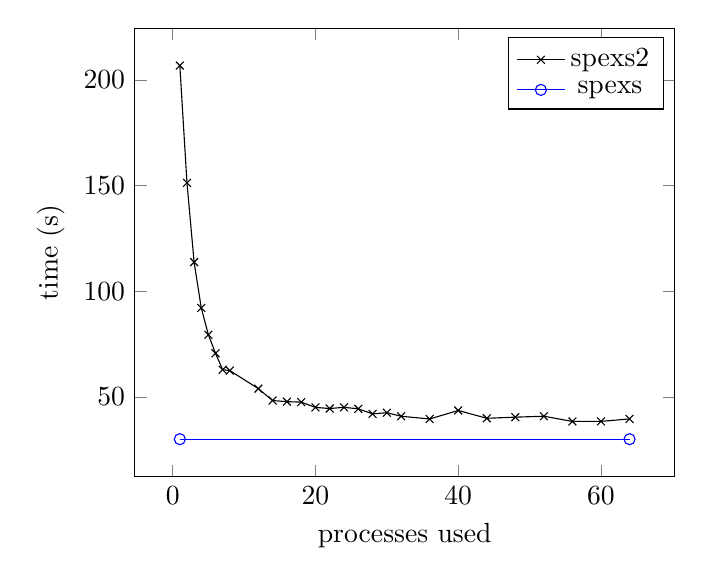
\begin{tikzpicture}
		\begin{axis}[xlabel=processes used, ylabel=time (s)]
			\addplot[color=black, mark=x] coordinates {
				(1, 206.81)
				(2, 151.30)
				(3, 113.80)
				(4, 92.16)
				(5, 79.42)
				(6, 70.66)
				(7, 62.89)
				(8, 62.49)
				(12, 53.93)
				(14, 48.30)
				(16, 47.77)
				(18, 47.56)
				(20, 45.06)
				(22, 44.53)
				(24, 45.09)
				(26, 44.39)
				(28, 41.99)
				(30, 42.55)
				(32, 40.87)
				(36, 39.58)
				(40, 43.61)
				(44, 39.91)
				(48, 40.44)
				(52, 40.89)
				(56, 38.41)
				(60, 38.45)
				(64, 39.61)
			};

			\addplot[color=blue, mark=o] coordinates {
				(1, 30.02)
				(64, 30.02)
			};

			\legend{spexs2, spexs}
		\end{axis}
	\end{tikzpicture}}
\subfloat[]{%
	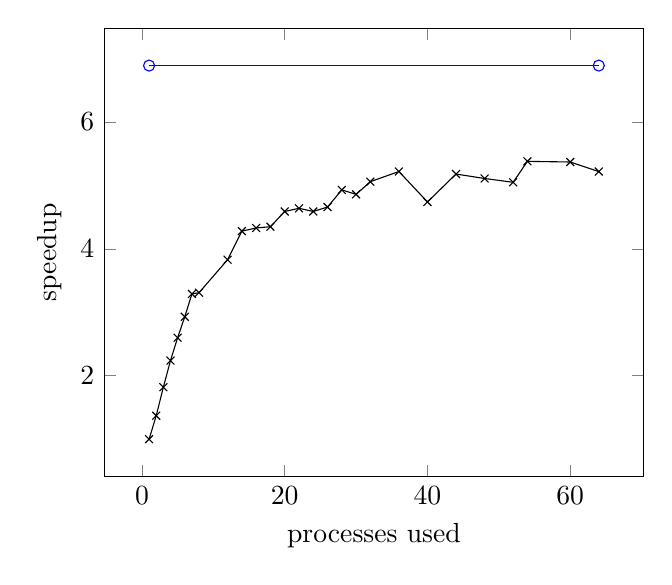
\begin{tikzpicture}
		\begin{axis}[xlabel=processes used, ylabel=speedup]
			\addplot[color=black, mark=x] coordinates {
				(1, 1.00)
				(2, 1.37)
				(3, 1.82)
				(4, 2.24)
				(5, 2.60)
				(6, 2.93)
				(7, 3.29)
				(8, 3.31)
				(12, 3.83)
				(14, 4.28)
				(16, 4.33)
				(18, 4.35)
				(20, 4.59)
				(22, 4.64)
				(24, 4.59)
				(26, 4.66)
				(28, 4.93)
				(30, 4.86)
				(32, 5.06)
				(36, 5.22)
				(40, 4.74)
				(44, 5.18)
				(48, 5.11)
				(52, 5.05)
				(54, 5.38)
				(60, 5.37)
				(64, 5.22)
			};

			\addplot[color=blue, mark=o] coordinates {
				(1, 6.89)
				(64, 6.89)
			};
		\end{axis}
	\end{tikzpicture}}
}
\end{figure}

The original \emph{spexs} works faster than \emph{spexs2} which is to be expected due to the runtime differences. At single core \emph{spexs2} performance is about 7 times slower than \emph{spexs}. We can expect 2x performance difference due to the Go runtime and compiler. The rest of the difference ~3.5x are most likely due to more general algorithm and some simplifications that were made to increase code readability.

The parallelization has significant benefit up to 20 cores. Amdahl's Law \cite{AmdahlsReval} states that the the parallel algorithms will be limited by their sequential parts; so this falloff is to be expected.

We showed that the algorithm benefits from parallelization although the runtime has significant impact on the performance of the program. Which suggests that \emph{spexs2} performance could be significantly improved with optimizations.